\chapter{Validação}\label{chp:LABEL_CHP_2}

Uma dificuldade que muitos alunos encontram na hora de escolher um tema para o projeto final para o curso de Graduação em Ciência da Computação é que, muitas vezes, não apenas desejam desenvolver um sistema que seja aplicável para a realização da sua colação de grau. Mas que o tema escolhido também possua uma aplicação com valor de negócio agregado e que seja utilizável por usuários realmente interessados e motivados.

Com essa preocupação, buscamos encontrar formas responsáveis de iniciar esse novo projeto, entendendo que seria necessário transformar a incerteza, de que teríamos um interesse significativo do público, em uma certeza. Para isso, antes de investir qualquer tempo no desenvolvimento dessa aplicação, buscamos encontrar uma forma de validar a nossa ideia inicial, de que construir um sistema para realizar testes de qualquer aplicação em produção na nuvem, era realmente uma ideia válida.

Existem diversas ferramentas que andam lado a lado com esse objetivo e ajudam a estruturar esse tipo de projeto, a que foi utilizada no projeto foi o Validation Board\cite{art:REF_ART_1}. Se trata em acompanhar o progresso do produto e focar no que realmente importa para o mesmo. É uma forma muito simples de descobrir se uma ideia vai funcionar ou se ela simplesmente não é válida, sendo totalmente baseada em ações e resultados rápidos.

\section{Validation Board}\label{sec:LABEL_CHP_2_SEC_A}

\begin{figure}
  \centering
  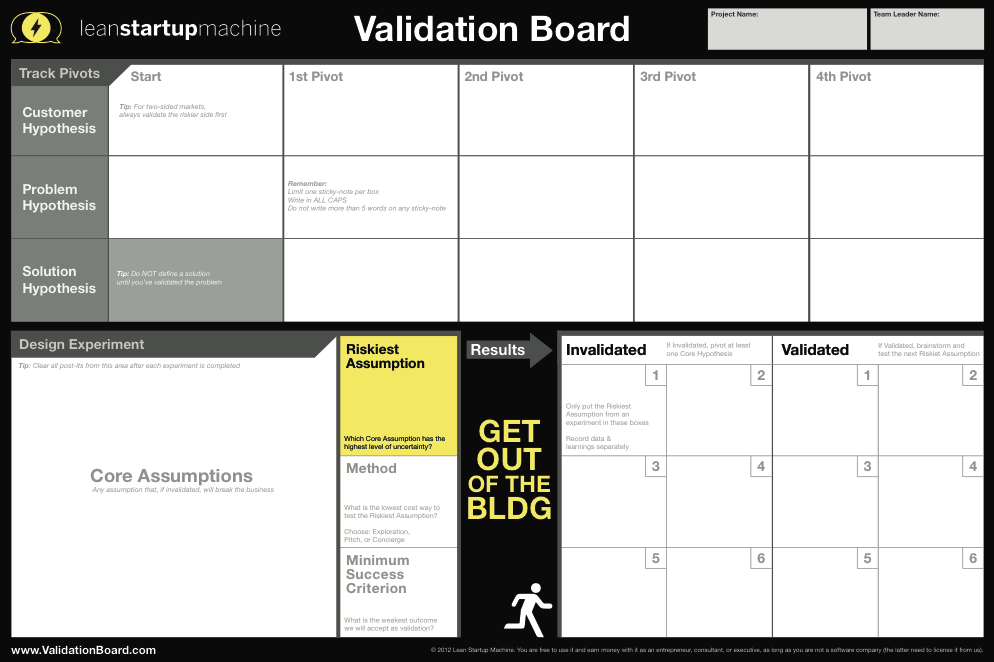
\includegraphics[width=0.6\textwidth]{imagens/validationTemplate.png}
  \caption{Validation Board}
  \label{fig:LABEL_FIG_1}
\end{figure}

O Validation Board foi desenvolvido pelo Lean Startup Machine, movimento formado por empreendedores do mundo todo que promove workshops de três dias que visa ensinar a construir algo que clientes tenham vontade de obter e também ensinam a executar experimentos que levem a sua empresa na direção certa. Ele é uma ferramenta simples e gratuita de testar as suas ideias, baseado na metodologia Lean\cite{art:REF_ART_2}.

O Validation Board consiste em criar hipóteses de determinado problema e de pessoas que sofrem do mesmo, gerando assim experimentos de constatação, ou não, dessas hipóteses. O objetivo é conseguir gerar aprendizado a partir da execução de cada um desses experimentos iterativamente, buscando sempre invalidar as hipóteses de maior para o menor risco, como por exemplo nos casos em que poderiam arruinar a ideia do seu produto.

Ao final de cada uma dessas iterações, temos dois resultados possíveis: a validação ou a invalidação da hipótese, e assim teremos insumos para tomar a próxima ação.

\subsection{A Hipótese}

O processo de validação é iniciado pelo topo do board, onde há espaço para diferentes pivôs. Pivôs são mudanças bruscas que não podem ocorrer na vida útil do produto no qual estamos aplicando esse processo. Primeiro definimos as hipóteses, são num total de três: Público Alvo, Problema e Solução. O público-alvo pode ser pensado como o grupo de pessoas que possui uma característica em comum. O problema deverá ser algo específico que esse grupo anterior possui. A solução é deixada em branco nessa primeira etapa. De forma a não ocultar outras  melhores oportunidades para resolver aquele problema. 

\subsection{Experimentações}

Na parte inferior do quadro, encontra-se a área de experimentação. Temos duas áreas: a de suposições iniciais onde deverão se encontrar as suposições que levam a acreditar que, se falharem, poderiam levar ao fracasso de todo o projeto; e a área de suposição de maior risco, que é a suposição a ser validada nessa iteração do processo.

\subsubsection {Métodos de teste}

A partir da suposição de maior risco, deve ser aplicado um experimento para provar a validade dessa suposição. Existem três métodos para isso:

\textbf{Exporation:} Neste método, o objetivo consiste em ir para as ruas e tentar reproduzir o problema que foi suposto na hipótese. Esse problema é algo real? Existem formas de resolvê-lo? Quais? Podem ser realizadas entrevistas com os usuários em potencial para, assim, identificar quais são as ideias que eles possuem a respeito de outras possíveis soluções para o problema também. Qualquer uma dessas atividades servem para prover insumos na hora de criar uma solução.

\textbf{Pitch:} O objetivo deste consiste no avaliador expor a ideia proposta para solucionar o problema e obter feedback dos usuários em potencial. De forma a descobrir o quanto eles pagariam, se pagariam, por utilizar essa solução e quanto.

\textbf{Concierge:} Este último método visa entregar ao cliente a sua hipótese de solução com a menor quantidade possível de desenvolvimento, de forma a fazê-los motivados com o produto que você tem a oferecer.

\subsubsection {Critério mínimo de sucesso}
Depois de definir qual será o método de teste a ser utilizado, é necessário definir quais serão os critérios que irão validar a sua ideia de fato, é muito importante que estes sejam definidos antes da aplicação do teste, para não viciar os seus resultados.

\subsection {Resultados}
Após toda a etapa de definição, deve-se "sair do prédio"  e realizar os experimentos necessários para a validação das premissas, conversando com pessoas reais de forma a por em prática o método de teste definido. 

A próxima fase consiste em determinar se os resultados alcançaram ou não o critério mínimo de sucesso, movendo a suposição para o campo validado ou invalidado. Caso ela seja invalidada, pode-se pivotar as hipóteses e reuniciar todo o processo. Caso contrário, o processo pode ser reiniciado com a próxima hipótese de maior risco, caso exista.

O Validation Board serviu como uma ótima opção para testar a nossa ideia, visto que ele torna possível acertar o quanto antes se o caminho a ser seguido é realmente o melhor, ou não.

\section{Aplicação do Validation Board}\label{sec:LABEL_CHP_2_SEC_B}

Com o Validation Board, desejávamos validar se o problema que estávamos buscando solucionar era realmente um problema, então seguimos as etapas da seguinte forma:

\subsection{Definião das hipóteses}
Definimos as três hipóteses: público alvo, problema e solução.

\textbf {Público alvo:} Grupo de desenvolvedores que tenham vontade em testar seus sistemas.

\textbf {Problema:} O grupo de desenvolvedores deseja testar seus sistemas mas possui algum empecilho.

\textbf{Solução:} Não definimos essa hipótese para não deixarmos de visualizar alguma outra possível solução para o problema.

\subsection{Definição das suposições}

Além das hipóteses, foram definidas suposições que nos levavam a acreditar que se falhassem, levariam ao fracasso da nossa ideia.

\textbf{Suposições iniciais:}
\begin{itemize}
\item É difícil configurar um ambiente de testes;
\item O custo de criar testes em projetos pequenos é alto;
\item O desenvolvedor não possui um ambiente próprio para executar os testes localmente;
\end{itemize}

\textbf{Suposição de maior risco:}
Desenvolvedores querem testar seus sistemas com uma ferramenta disponível na nuvem.

\begin{figure}
  \centering
  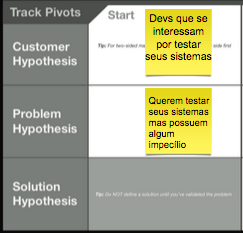
\includegraphics[width=0.6\textwidth]{imagens/hyphotesis.png}
  \caption{Hipóteses definidas no Validation Board}
  \label{fig:LABEL_FIG_2}
\end{figure}

\begin{figure}
  \centering
  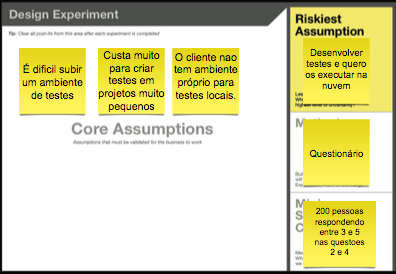
\includegraphics[width=0.6\textwidth]{imagens/assumptions.png}
  \caption{Suposições definidas no Validation Board}
  \label{fig:LABEL_FIG_3}
\end{figure}

\begin{figure}
  \centering
  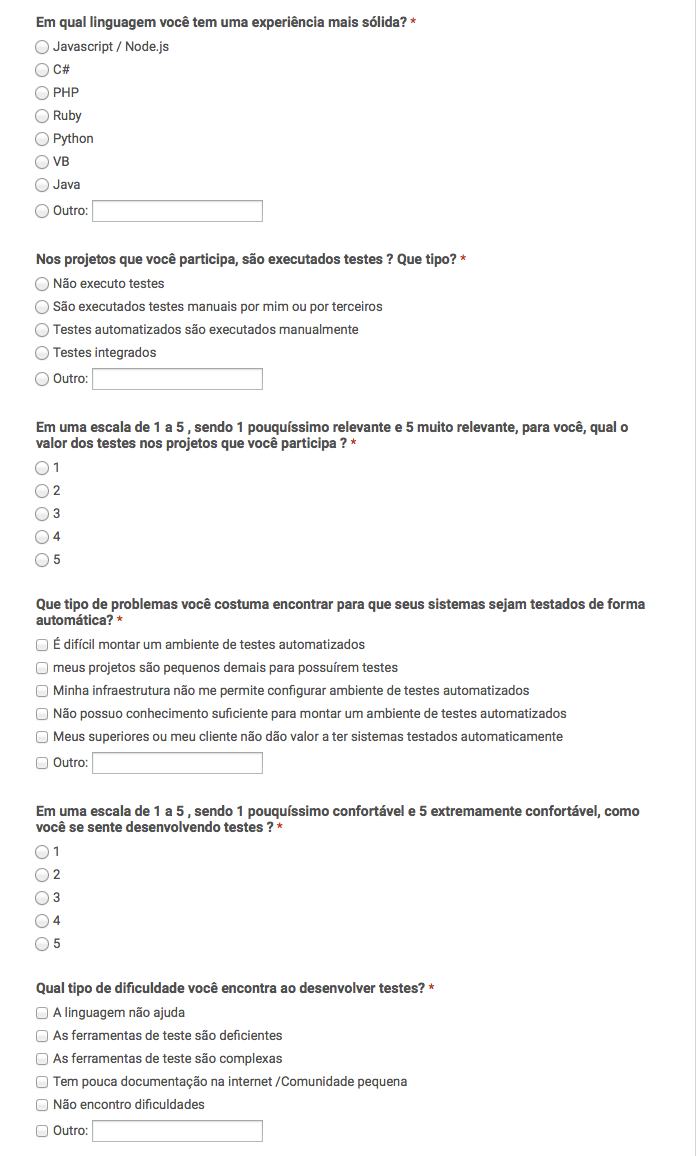
\includegraphics[width=0.8\textwidth]{imagens/survey.png}
  \caption{Pesquisa aplicada ao público alvo}
  \label{fig:LABEL_FIG_4}
\end{figure}

\subsection{Experimentação}

Para realizar as nossas experimentações, definimos o método de teste \emph{Exploration}, onde criamos um formulário com perguntas a serem aplicadas nos nossos possíveis clientes. Utilizamos como canal de aplicação dessa pesquisa grupos de desenvolvedores no Facebook (NodeJS Brasil, Angular Brasil, Javascript Brasil, Javascript Brasil, etc).

\subsubsection{Pesquisa}
A pesquisa foi formulada com um conjunto de perguntas que julgamos interessantes para identificar o perfil do desenvolvedor brasileiro, e por consequência, validar a nossa hipótese.

\subsubsection{Critério mínimo de sucesso}


\section {Resultados}

